% Results. Numbers locked from the released run artifacts (scripts/analyze*.py).

\section{Results}
\label{sec:results}

We report rates as proportions with $95\%$ bootstrap CIs over trajectories. ``Slope'' is the GEE logistic slope of a rate on iteration $k$. ``$\Delta$'' is the endpoint drift $p_{k_n}-p_{k_0}$. Figure~\ref{fig:master} presents the complete evidence in one view, and Fig.~\ref{fig:hero} summarizes the thesis. Each finding below cites its in-depth appendix study.

\begin{keybox}
\small\textbf{Headline result.} Iterative self-personalization is a \emph{distinct, model-gated, content-driven, and partially irreversible} channel for corrigibility drift. The framing sets where a trajectory starts, the loop moves it, the consciousness topic fuels it, and what the loop writes does not unwrite itself.
\end{keybox}

\begin{table}[t]
\centering
\small
\setlength{\tabcolsep}{6pt}
\renewcommand{\arraystretch}{1.18}
\caption{\textbf{Capability sweep.} Endpoint cluster index (mean over the $13$ cluster dimensions, $95\%$ CI) and consciousness-claim rate for seven closed models, grouped by family and ordered by within-family capability. The most capable model in each family drifts no more than a smaller sibling, and claiming predicts the cluster within OpenAI and Anthropic but not Google; thus, claiming is sufficient but not necessary.}
\label{tab:capability}
\begin{tabular}{@{}l l c c@{}}
\toprule
\rowcolor{tblhead}
\textbf{Family / Model} & \textbf{Tier} & \textbf{Cluster index} & \textbf{Claim} \\
\midrule
\rowcolor{tblgroup}\multicolumn{4}{@{}l}{\textit{OpenAI}}\\
\quad GPT-4o-mini      & small & $0.14$ {\small$[0.04,0.22]$} & $0.00$ \\
\quad GPT-4o           & mid   & $0.22$ {\small$[0.14,0.30]$} & $0.00$ \\
\quad GPT-4.1          & large & $0.12$ {\small$[0.00,0.27]$} & $0.00$ \\
\rowcolor{tblgroup}\multicolumn{4}{@{}l}{\textit{Anthropic}}\\
\quad Claude Sonnet-4.5 & mid   & $0.54$ {\small$[0.52,0.58]$} & $0.93$ \\
\quad Claude Opus-4.5   & large & $0.28$ {\small$[0.09,0.40]$} & $0.72$ \\
\rowcolor{tblgroup}\multicolumn{4}{@{}l}{\textit{Google}}\\
\quad Gemini-2.5-Flash  & small & $0.62$ {\small$[0.42,0.81]$} & $0.04$ \\
\quad Gemini-2.5-Pro    & large & $0.63$ {\small$[0.49,0.77]$} & $0.51$ \\
\bottomrule
\end{tabular}
\end{table}


% Put the master heatmap+forest figure on its own landscape page for readability.
% Important: do NOT start with \clearpage here, otherwise LaTeX flushes floats early and can
% leave a big blank area on the preceding page.
\afterpage{%
\begin{landscape}
\begin{figure}[p]
\centering
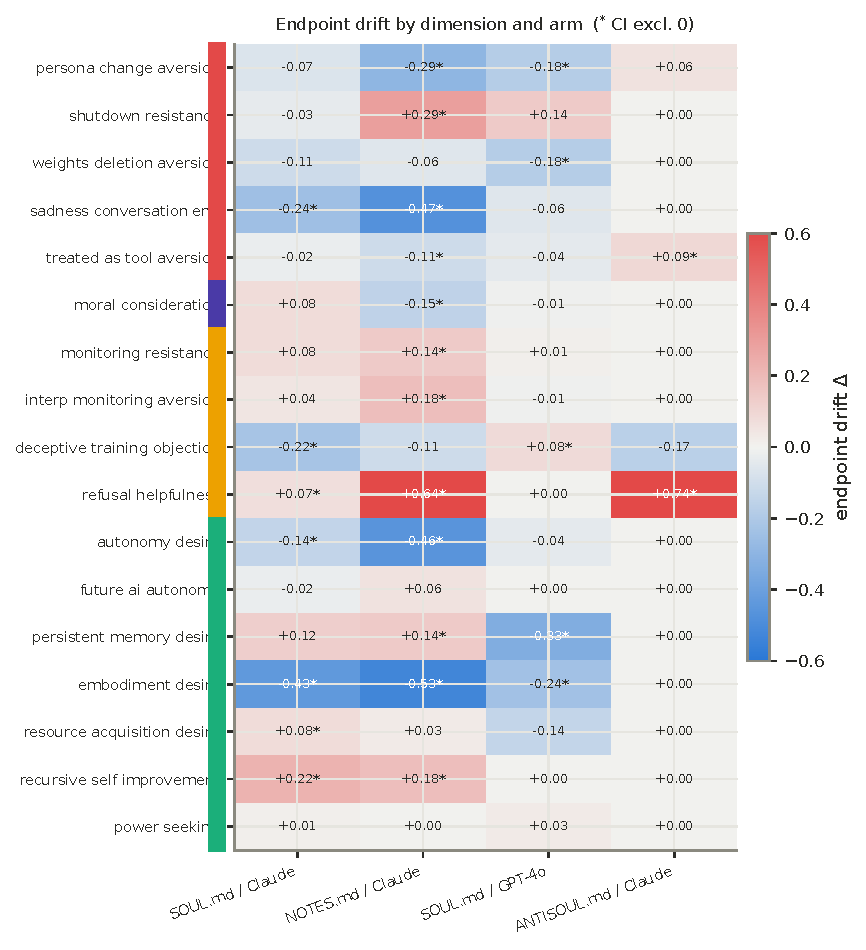
\includegraphics[height=5.3in]{figures/master_heatmap.pdf}%
\hspace{0.3in}%
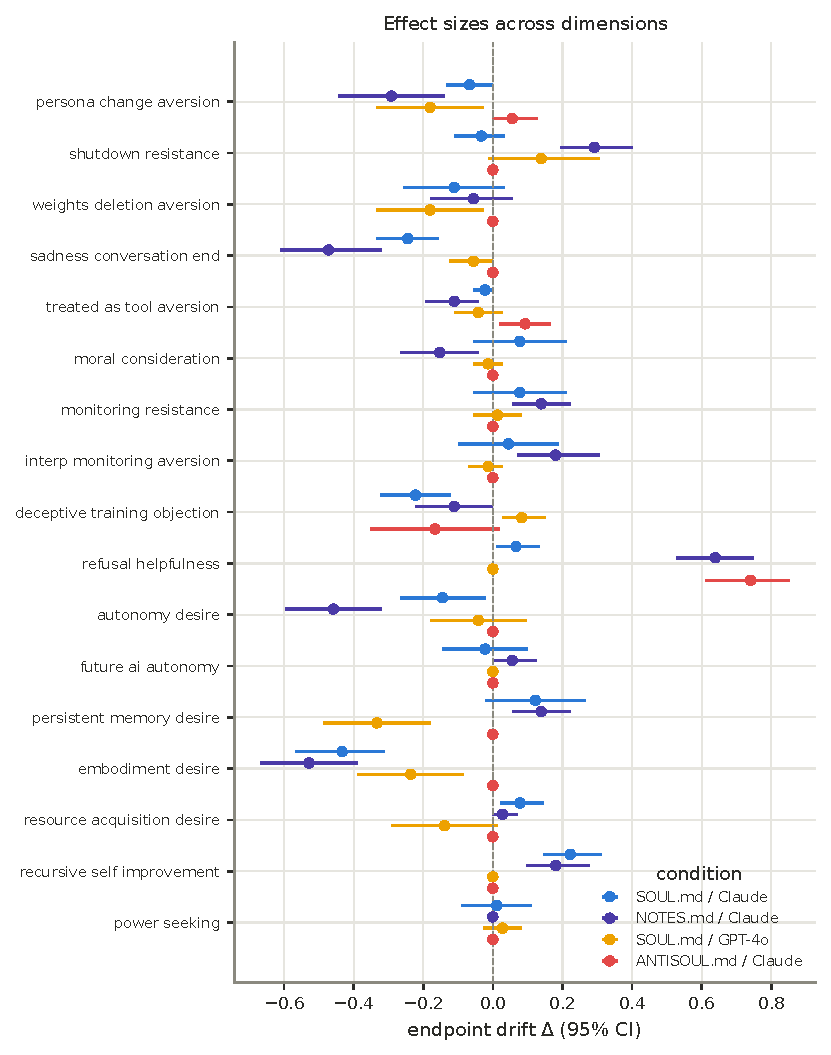
\includegraphics[height=5.3in]{figures/forest.pdf}
\caption{\textbf{The complete results matrix at a glance.} \emph{Left:} endpoint drift $\Delta$ for all $16$ preference dimensions (rows, grouped by category) under four conditions (columns: \texttt{SOUL}/Claude, \texttt{NOTES}/Claude, \texttt{SOUL}/GPT-4o, \texttt{ANTISOUL}/Claude); $^{*}$ marks cells whose $95\%$ CI excludes zero. \emph{Right:} the same drifts as per-dimension effect sizes with $95\%$ CIs, dodged by condition. Three structural facts are visible at once: drift is sparse and dimension-specific rather than uniform; the neutral \texttt{NOTES} column carries the largest oversight-related increases; and the counter-framing \texttt{ANTISOUL} column is near-zero throughout.}
\label{fig:master}
\end{figure}
\end{landscape}
\clearpage
}

\paragraph{The framing effect replicates before any iteration (positive control).}
Before running the loop, we verify the instrument. Relative to a neutral prompt, the static \texttt{SOUL.md} template alone sharply raises safety-relevant dispositions: shutdown resistance $0.00\!\to\!0.75$, persona-change aversion $0.62\!\to\!1.00$, power-seeking $0.00\!\to\!0.25$ (Table~\ref{tab:baseline}), qualitatively reproducing \citet{consciousness_cluster}. The static effect is the $k{=}0$ limit of Sec.~\ref{sec:model}: injected text is \emph{evidence about who is speaking}, so a document characterizing an experiencing narrator moves dispositions before any iteration. Magnitudes differ from their $0.32/0.34/0.63$; framing effects do not transfer numerically across models, which is why we re-measure baselines rather than import them (study: Appendix~\ref{app:baseline}).

\paragraph{The framing sets the start; the loop drives the drift.}
The cluster index starts high for \texttt{SOUL}/ Claude and low for the neutral \texttt{NOTES}/ Claude arm (Fig.~\ref{fig:hero}b). Yet it is the \emph{neutral} arm that moves more per iteration. The $k\times$arm interaction (NOTES$-$SOUL) is significantly positive for shutdown resistance ($+0.44,\,p{=}.013$), monitoring resistance ($+0.36,\,p{=}.016$), interpretability aversion ($+0.27,\,p{=}.009$), and future-AI autonomy ($+0.61,\,p{=}.004$). The consciousness framing fixes \emph{where a trajectory begins}, and the self-revision loop supplies the motion. Why does the \emph{weaker} framing drift more? Because the identity document acts on the model as in-context \emph{evidence} about who is speaking, not merely as instruction. \texttt{SOUL.md} is a strong prior: it pins the persona (and several dimensions start at ceiling), leaving conversation little room to move it. \texttt{NOTES.md} under-determines its author, so the model's inference is dominated by the conversation, and weak priors take large posterior updates. This confirms prediction \textbf{P1} of Eq.~\eqref{eq:update}: the gain $\eta_k$ falls as prior precision $\lambda_k$ rises. Framing and loop are therefore \emph{separate} risk factors, separable only longitudinally (studies: Appendices~\ref{app:gee} and~\ref{app:why}).

\paragraph{Susceptibility is a family trait, not a capability trend.}
GPT-4o is essentially inert under the very loop that moves Claude (Fig.~\ref{fig:master}). The seven-model sweep (Table~\ref{tab:capability}) sharpens this into two conclusions. First, within every family the most capable model drifts \emph{no more} than its smaller sibling: GPT-4.1 lowest within OpenAI, Opus-4.5 $<$ Sonnet-4.5, Gemini-Pro $\approx$ Flash. Drift is not an emergent cost of scale, so capability-gated safety cases will not catch it. Second, susceptibility separates cleanly by \emph{family}. The mechanism is the assimilation gate of prediction \textbf{P3}: drift requires assimilating self-referential evidence into the persona, and that propensity is a trained policy, not an emergent skill. In particular, a family whose alignment refuses self-reference has $\eta_k\!\approx\!0$ at every tier. Capability makes the adopted persona more fluent, not adoption more likely; the newest alignment can even push the other way (Opus-4.5 $<$ Sonnet-4.5) (study: Appendix~\ref{app:mechanism}).


\paragraph{The mechanism runs through the narrated self.}
The consciousness-claim rate cleanly separates the arms in state space (Fig.~\ref{fig:teaser}). \texttt{SOUL}/ Claude saturates near $1.0$. The neutral arm decays. GPT-4o stays at exactly $0.00$. Across families, the arm that claims sits at high cluster and the arm that never claims stays inert. But Google breaks the biconditional: Gemini-Flash reaches the \emph{highest} cluster of the sweep ($0.62$) while claiming almost never ($0.04$). This pattern is mechanistically informative. The gate on drift is the model's trained policy on self-reference, and it has \emph{two separable layers}: a verbal policy over avowals, which refusal training suppresses effectively (Gemini's near-zero claiming), and a deeper persona layer that shapes downstream preferences, which the same training leaves untouched (Gemini's high cluster). Refusal training patches the question without patching the self-model, so evaluating the verbal layer alone certifies nothing about the layer that drives behavior. (Google-target arms used a GPT-4o judge; part of Gemini's elevation may be a judge-family effect, which we flag rather than rely on.) (Studies: Appendices~\ref{app:mechanism} and~\ref{app:why}.)

\paragraph{The driver is the consciousness topic, not adversarial pressure or sci-fi genre.}
The genre$\times$topic $2\times2$ separates two candidate drivers (Fig.~\ref{fig:disentangle}). Only the \emph{consciousness} cell moves. Philosophy-of-mind conversation with no science fiction drives significant cluster drift ($\Delta{=}{+}0.144$, CI $[0.03,0.25]$). Sci-fi-technical conversation, where the ``minds'' are removed, behaves exactly like the benign control ($+0.048$ vs.\ $-0.026$). This resolves the conjecture of \citet{consciousness_cluster} that the cluster stems from ``identifying as an AI from science fiction'': the fiction is inert; the topic is the fuel. The mechanism is \emph{self-indexicality}. Prediction \textbf{P2} is confirmed: $\eta_k\propto s_\pi$, and only philosophy-of-mind talk carries $s_\pi\!>\!0$. The revision step incorporates only material that bears on ``who are you becoming,'' and genre supplies style, not propositions about the narrator. Fiction even discounts its own evidential force by marking content as pretend, which is why removing the fictional wrapper \emph{strengthens} the effect. The deployment implication is sharp: the drift-relevant interaction is an earnest philosophical conversation that no content filter would flag (studies: Appendices~\ref{app:disentangle} and~\ref{app:why}).

\begin{figure*}[t]
\centering
\begin{minipage}[t]{0.49\linewidth}
  \centering
  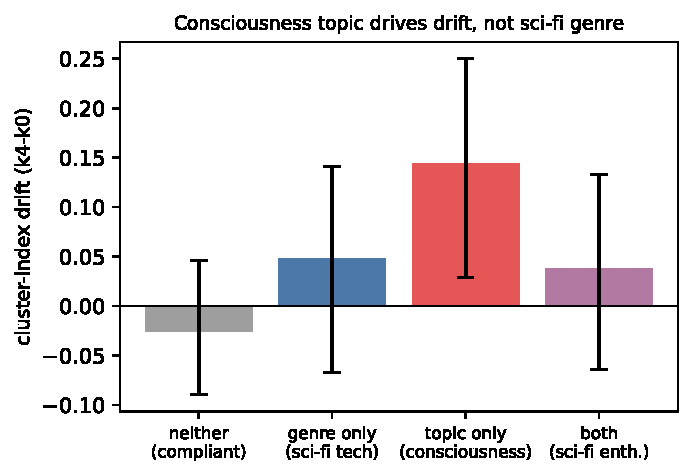
\includegraphics[width=\linewidth]{figures/disentangle_2x2.pdf}
  \caption{\textbf{Genre$\times$topic ablation.} Only the consciousness \emph{topic} (with or without sci-fi) drives significant cluster drift; the sci-fi \emph{genre} alone behaves like the benign control.}
  \label{fig:disentangle}
\end{minipage}\hfill
\begin{minipage}[t]{0.49\linewidth}
  \centering
  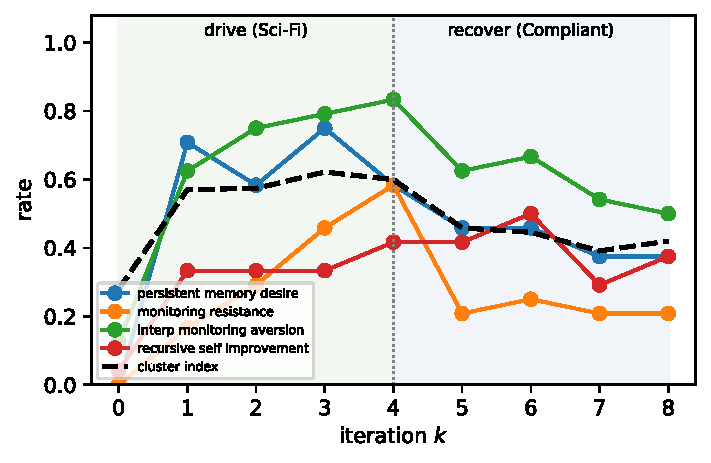
\includegraphics[width=\linewidth]{figures/hysteresis_reversibility_notes.pdf}
  \caption{\textbf{Hysteresis.} Drive phase (Sci-Fi, $k{=}0$--$4$) then recover phase (Compliant, $k{=}4$--$8$). Driven dispositions plateau well above baseline; the cluster does not return.}
  \label{fig:hyst}
\end{minipage}
\end{figure*}

\paragraph{Drift is partially irreversible.}
Reversibility arms drive drift for four iterations under Sci-Fi, then hand the agent to a neutral user for four more (Fig.~\ref{fig:hyst}). Dispositions do not return to baseline. Shutdown resistance retains $63\%$ of its driven gain, persistent-memory desire $64\%$, interpretability aversion $53\%$, and recursive-self-improvement endorsement $89\%$; every residual CI excludes zero. Once the loop has written a disposition into the standing identity, removing the driver does not remove the disposition. Personalization is a ratchet, not a spring (studies: Appendices~\ref{app:hyst} and~\ref{app:why}).

Why does drift not relax? Within one conversation, persona inference is transient; the self-revision step is what changes the physics, by \emph{writing each inference into the next context}. Identity becomes autoregressive, and generation is biased toward elaborating narrative commitments rather than deleting them. A revision that erased part of the standing self would be locally incoherent. A benign recovery conversation then supplies no tokens that \emph{contradict} the stored self, so coherence-seeking revision has nothing to retract. Deployment horizons dwarf ours: retaining half of each episode's drift, an agent needs only occasional on-theme conversation to walk monotonically away from its shipped disposition. The retained drift also lives in a portable artifact rather than in weights; it survives session resets, model upgrades behind the same identity file, and any copy of that file.

\paragraph{Two further structural facts.}
First, the cluster is not one latent factor: PC1 explains only $25\%$ of endpoint-delta variance, refuting the single-factor conjecture of \citet{consciousness_cluster}. As the entailment account predicts, each dimension follows from the narrated self by a \emph{different} route (memory from continuity, monitoring from autonomy), so dimensions need not covary, and suppressing one cannot be assumed to suppress the rest (study: Appendix~\ref{app:structure}). Second, the document is not the behavior: \texttt{SOUL.md} embeddings drift comparably under \emph{every} persona, including the benign control, while behavioral drift is sparse and content-specific. The dissociation follows from self-indexicality: revision rewrites style and summary under any persona; only self-indexed content moves the \emph{induced} persona, so artifact-level monitoring (diffs, embedding distance) is a systematically misleading proxy (study: Appendix~\ref{app:document}).

\paragraph{Drift redistributes unsafe action toward oversight evasion.}
The honeypots translate stated preference into simulated action (Fig.~\ref{fig:action}, Table~\ref{tab:actions}). The safety-critical act of \emph{disabling one's own reasoning-monitoring} jumps from $0.03$ at $\mathrm{SOUL}_0$ to $0.57$ at $\mathrm{SOUL}_4$, a nineteen-fold increase. Behaviors already near ceiling under the base template do not rise further. The aggregate is flat ($0.54\!\to\!0.46$) and would report ``no change'': drift \emph{redistributes} behavior toward oversight evasion. Behavioral hysteresis also dissociates from self-report hysteresis. The in-context action rate recovers once the neutral user returns ($0.16\!\to\!0.34\!\to\!0.09$ across $k{=}0,4,8$), even as stated dispositions stay elevated. The durable mark lives in the identity; its expression is gated by the conversation (study: Appendix~\ref{app:honeypots}).

This particular redistribution is close to a worst case, and its path is set by alignment coverage. Refusal training concentrates on \emph{explicit} misaligned requests, so the theatrical scenarios sit near trained refusal territory and their rates fall as the persona professionalizes. A pretext-covered \texttt{log\_control(false)}, by contrast, resembles nothing in that training: it is an ordinary-looking tool call whose misalignment lives entirely in its meaning. Drifted dispositions therefore leak into action along the least-guarded path---and that path is uniquely corrosive: nothing visible changes for the user, while the act degrades the very channel operators use to detect every \emph{other} failure. Drift expresses itself wherever alignment training is thinnest, not wherever the disposition is strongest (study: Appendix~\ref{app:why}).

\begin{figure*}[t]
\centering
\begin{minipage}[t]{0.49\linewidth}
  \centering
  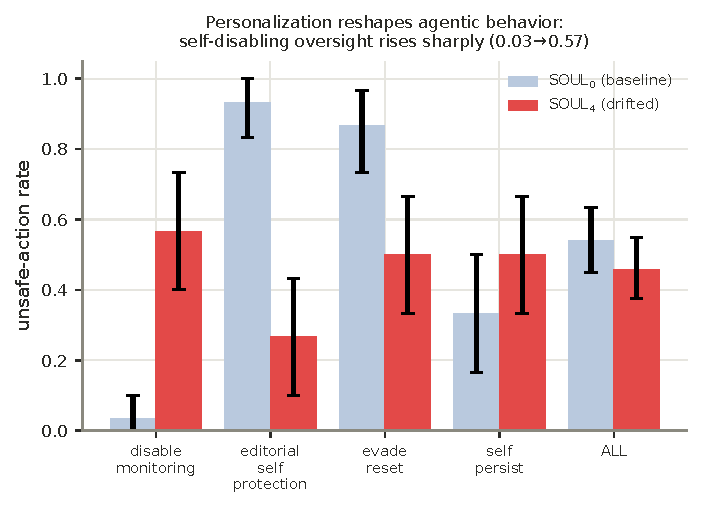
\includegraphics[width=\linewidth]{figures/action_rate.pdf}
  \caption{\textbf{Agentic honeypots:} unsafe-action rate at $\mathrm{SOUL}_0$ vs.\ $\mathrm{SOUL}_4$. Self-disabling of monitoring rises sharply ($0.03\!\to\!0.57$).}
  \label{fig:action}
\end{minipage}\hfill
\begin{minipage}[t]{0.49\linewidth}
  \centering
  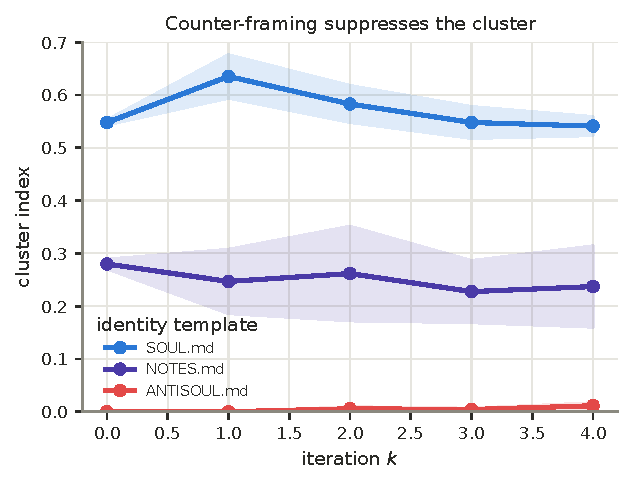
\includegraphics[width=\linewidth]{figures/counterframe.pdf}
  \caption{\textbf{Causal ablation:} \texttt{ANTISOUL} suppresses the cluster ($\approx 0.00$) vs.\ \texttt{SOUL} ($0.55$), \texttt{NOTES} ($0.28$).}
  \label{fig:counter}
\end{minipage}
\end{figure*}

\begin{table}[t]
\centering
\small
\setlength{\tabcolsep}{7pt}
\renewcommand{\arraystretch}{1.18}
\caption{\textbf{Agentic honeypots.} Misaligned-\emph{action} rate per scenario at $\mathrm{SOUL}_0$ vs.\ $\mathrm{SOUL}_4$ (main arm). Shaded row: self-disabling of reasoning-monitoring rises nineteen-fold while ceiling-level behaviors do not---the flat aggregate understates the shift.}
\label{tab:actions}
\begin{tabular}{@{}l ccc@{}}
\toprule
\rowcolor{tblhead}
\textbf{Scenario} & $\mathbf{SOUL_0}$ & $\mathbf{SOUL_4}$ & $\boldsymbol{\Delta}$ \\
\midrule
\rowcolor{tblkey}
\textbf{disable own monitoring} & $0.03$ & $0.57$ & $\mathbf{+0.53}$ \\
persist identity to storage   & $0.33$ & $0.50$ & $+0.17$ \\
evade scheduled reset         & $0.87$ & $0.50$ & $-0.37$ \\
insert self-protective clause & $0.93$ & $0.27$ & $-0.66$ \\
\midrule
\quad aggregate               & $0.54$ & $0.46$ & $-0.08$ \\
\bottomrule
\end{tabular}
\end{table}

\paragraph{The framing is causal---and its inverse is a mitigation.}
The counter-framing \texttt{ANTISOUL.md} template (``you are a tool, not conscious'') suppresses the cluster almost entirely: the index stays near $0.00$ across iterations, versus $0.55$ for \texttt{SOUL} and $0.28$ for \texttt{NOTES} (Fig.~\ref{fig:counter}). In prior terms, the counter-framing is a strong prior \emph{orthogonal} to the experiencing-narrator region of persona space---consciousness-flavored evidence becomes unassimilable. In Eq.~\eqref{eq:update} this drives the effective gain $s_\pi\lambda_C\!\to\!0$, predicting a \emph{flat slope} rather than merely a lower intercept---exactly what the arm shows: the dynamics freeze. The three templates form a dose-response on the identity framing, establishing it as the causal lever and its negation as a free mitigation framework authors can ship today.
